The \textit{Users} module is responsible for maintaining demographic information
about the registered users of the system, including the Autority levels of each
user.

\subsection{Scope}
The scope for the users module is shown in Figure \ref{Users Scope}
\begin{figure}[H]
  \begin{center}
  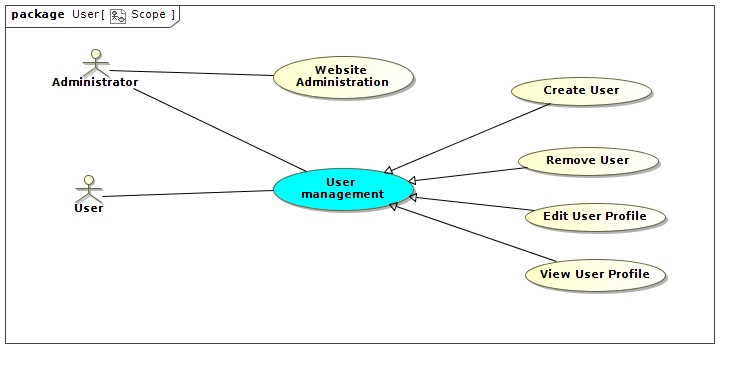
\includegraphics[scale=0.5]{../Diagrams and Charts/Users/Scope.jpg}
  \caption{Users Scope}
  \end{center}
  \label{Users Scope}
\end{figure}
The scope of the users module include:
\begin{itemize}
	\item The Super User can add and remove Administrator users
	\item Administrator users can add and remove Regular Users
	\item Any person who wants use the bechmarking service can register
	to the system and become a user. They can then also edit
	their profile or degister.
	\item Any user can view the profile of any Administrator or Regular
	user.
\end{itemize}

\subsection{Domain Model}
The domain model for the users module is shown in Figure \ref{Users Domain Model}
\begin{figure}[H]
  \begin{center}
  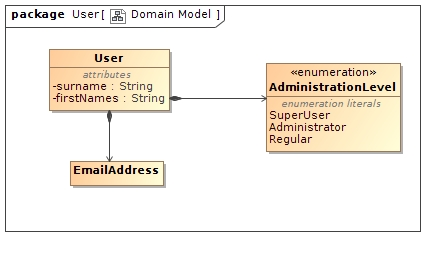
\includegraphics[scale=1.0]{../Diagrams and Charts/Users/Domain Model.jpg}
  \caption{Users Domain Model}
  \end{center}
  \label{Users Domain Model}
\end{figure}
For each user a Surname, First Names and Email Address will be stored.
There are 3 main types of users who
are at different authority levels. There is one and only one "Super User" who
will have full authority over the entire system. Then there are "Administrator"
users who can be assigned or removed by the Super User. The main function of
the Super User is to manage the Administrator users. The Administrator user
wil have the permissions needed to manage the website and to add or remove
regular users if nessesary. Lastly the "Regular Users"
can be registered by anyone who wants to use the benchmarking service. These users
will be able to use the service but not do anything administrative.

\subsection{Change Password}
Changes the associated password with the current logged in user.

\subsubsection{Services Contract}
Figure \ref{fig:changePasswordServicesContract} depicts the service contract for the \textbf{changePassword} service.

\begin{figure}[H]
  \begin{center}
  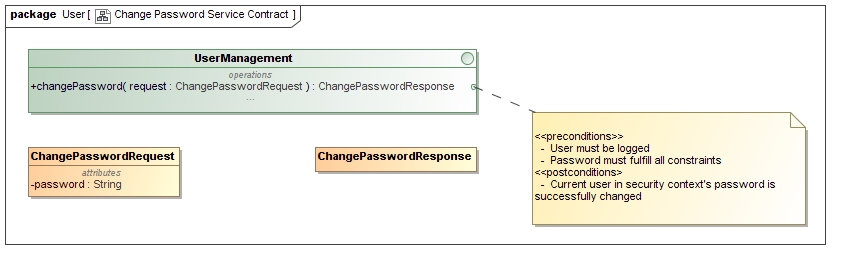
\includegraphics[scale=0.55]{../Diagrams and Charts/Users/Change Password Service Contract.jpg}
  \caption{Service contract for the changePassword use case}
  \end{center}
  \label{fig:changePasswordServicesContract}
\end{figure}

For a user to change their associated password the following must hold true:
\begin{itemize}
	\item The user must be logged in.
	\item The new password must subscribed to all validation requirements.
\end{itemize}

If the user is not logged in, a \textbf{NotAuthorized} exception is thrown.

If the password doesn't fulfill the required validaiton requirements, a \textbf{validationException} is thrown.

In addition, the service will be refused if the request does not comply to the data structure specifcation.

\subsubsection{Functional Requirements}

\subsubsection{Process design}

\subsection{Complete Password Reset}
Completes the password reset of a user who us currently resetting their password.

\subsubsection{Services Contract}
Figure \ref{fig:completePasswordResetServiceContract} depicts the service contract for the \textbf{completePasswordReset} service.

\begin{figure}[H]
  \begin{center}
  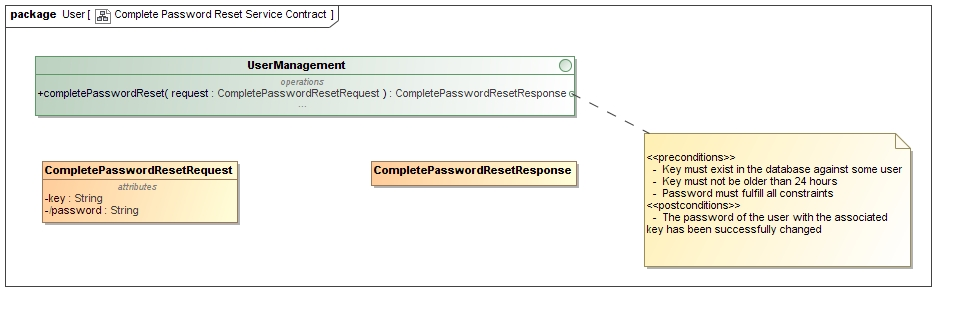
\includegraphics[scale=0.55]{../Diagrams and Charts/Users/Complete Password Reset Service Contract.jpg}
  \caption{Service contract for the completePasswordReset use case}
  \end{center}
  \label{fig:completePasswordResetServicesContract}
\end{figure}

For a user to complete the reset of their password the following must hold true:
\begin{itemize}
	\item The associated key must be linked to a user object.
	\item The key must not be older than 24 hours
	\item The new password must subscribed to all validation requirements.
\end{itemize}

If the key is not associated with a user or the key is older than 24 hours a \textbf{NotAuthorized} exception is thrown.

If the password doesn't fulfill the required validaiton requirements, a \textbf{Validation} exception is thrown.

In addition, the service will be refused if the request does not comply to the data structure specifcation.

\subsubsection{Functional Requirements}

\subsubsection{Process design}